\chapter{Fundamentação Teórica}

\section{Redes Definidas por Software}

De acordo com a \citeonline{SDNFoundation} e \citeonline{ALSMADI}, o paradigma SDN é uma arquitetura emergente que se diferencia por ser  dinâmica, gerenciável, de bom custo-benefício e com boa adaptabilidade, o que a torna ideal para aplicações que exigem alta largura de banda e ainda pela natureza dinâmica dessas aplicações.
\par A arquitetura SDN possui como principais características:

\begin{itemize}
    \item \textbf{Diretamente programável}: O controle da rede é diretamente programável devido a seu desacoplamento das funções de encaminhamento;
    \item \textbf{Ágil}: A abstração do controle de encaminhamento de pacotes por meio dos controladores permite que os administradores ajustem dinamicamente o fluxo de tráfego;
    \item \textbf{Gerenciamento Centralizado}: A inteligência lógica da rede é centralizada nos controladores, que possuem uma visão global da rede;
    \item \textbf{Programaticamente Configurável}: SDN permite que os administradores configurem, gerenciem, e otimizem sua segurança rapidamente via aplicações automatizadas para SDN, independente de softwares proprietários;
    \item \textbf{ Baseada em padrões abertos}: A implementação SDN em padrões abertos simplifica o projeto e a operação de redes.
    \item \textbf{Gerenciamento baseado em fluxos:}  Apesar do controle por fluxo também existir nas redes convencionais, os protocolos de roteamento se baseiam nos endereços IP para a tomada de decisões. Para o SDN, as decisões de encaminhamento tomam como base os fluxos que entram e saem dos \emph{switches}.
    
\end{itemize}

\subsection{Histórico}
O surgimento das Redes Definidas por Software remonta anos de pesquisas em diversas tecnologias de redes e seus paradigmas. Cada pesquisa, desejando compreender ou solucionar algum problema específico na área de redes terminou por contribuir para o desenvolvimento do que hoje chamamos de redes SDN (\textit{Software-Defined Networking}).

\begin{figure}[!h]
	\caption{ Desenvolvimento de redes programáveis com o passar dos
	anos.
}
  \centering
  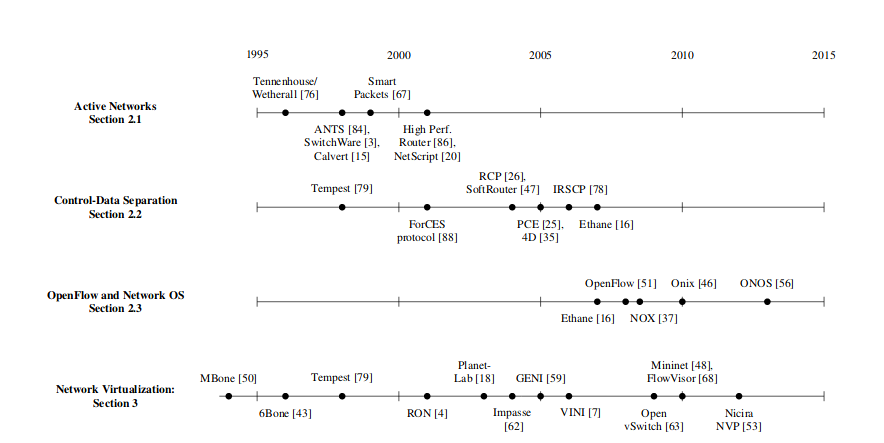
\includegraphics[scale=0.5]{Imagens/SDNHistory(1).png} 
  
  \legend{Fonte:\citeonline{Feamster:2013:RS:2559899.2560327} }
  \label{SDNHistory(1).png}
\end{figure}

\par A história do paradigma SDN, observando a Figura \ref{SDNHistory(1).png}, se inicia com o estudo de redes ativas e virtualização de redes durante os anos 90, período no qual a internet se tornou escalável e crescia rapidamente\cite{Feamster:2013:RS:2559899.2560327}.
De acordo com \citeonline{Tennenhouse:1997:SAN:2288390.2288938,Bhattacharjee:1997:AAN:267213.267289}, as redes ativas podem ser definidas como redes que possuem capacidade de expor recursos dos nós e customizar a computação de dados que passam pelos \textit{switches}, funcionalidades até então inexistentes nas redes convencionais passivas. Nesse mesmo período as pesquisas de virtualização de redes também avançavam e sua importância se dá porque a virtualização abstrai o funcionamento de uma rede, desacoplando-a da infraestrutura física de forma a diminuir a complexidade sobre a mesma. 
\par Por volta dos anos 2000, o volume de tráfego de rede continuava aumentando, e os pesquisadores buscavam balancear esse aumento de tráfego com características como confiabilidade, previsibilidade e performance da rede. Entretanto, o principal obstáculo se encontrava na integração inflexível entre o plano de controle e de dados nos roteadores e \emph{switches} convencionais. Essa integração dificultava  a exploração de novos protocolos nas redes, tornando os administradores dependentes do suporte da infraestrutura física. A partir de então outros estudos foram feitos para separar essas duas camadas, gerando inovações como a abertura de interface entre os planos de controle e de dados e também através de novas arquiteturas com centralização da lógica do controle da rede. Essas inovações são vistas respectivamente através da interface ForCES(\textit{Forwarding and Control Element Separation}) e das arquiteturas RCP (\textit{Rounting Control Protocol}) e SoftRouter.
\cite{Nunes}
\par A partir de 2005, a separação do plano de controle do plano de dados já era uma realidade, contudo, ainda era necessário experimentos em larga escala para validar as vantagens e desvantagens dessa separação, dessa forma, os campus das universidades se tornaram ambientes de experimentação de novas arquiteturas e protocolos. 
Uma das arquiteturas propostas nessa 
Proposto por \citeonline{Casado} e também desenvolvido na Universidade de Stanford, a arqui
Nesse contexto, foi desenvolvido na Universidade de Stanford em 2008 um protocolo aberto de comunicação entre o controlador da rede e a infraestrutura física, tornando as redes SDN finalmente viáveis: o protocolo OpenFlow\cite{McKeown:2008:OEI:1355734.1355746}.



O OpenFlow é sucessor do padrão Ethane, proposto por \citeonline{Casado} e  também desenvolvido na Universidade de Stanford. Sua proposta consistia de dois elementos: o \emph{switch} Ethane, que possuía uma tabela de fluxos e um canal seguro de comunicação com o controlador; e o próprio controlador, que tomava decisões sobre o encaminhamento dos pacotes.  

\subsection{Arquitetura SDN}

  A arquitetura SDN pode ser descrita de forma simplificada como na Figura \ref{SDN.png}. Os \emph{switches} e roteadores ligados aos sistemas finais se comunicam com o controlador SDN de forma que este possa ter uma visão global da rede e tome decisões dinamicamente com base no estado atual da rede, repassando estas decisões aos elementos físicos.

   \begin{figure}[!h]
	\caption{ Elementos da arquitetura SDN}
  \centering
  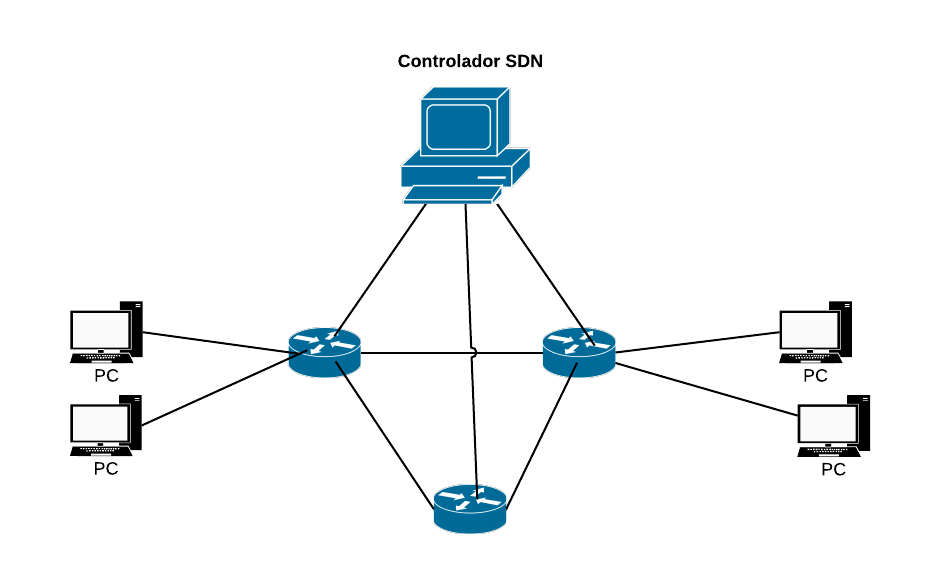
\includegraphics[scale=0.3]{Imagens/SDN.png} 
 
  \legend{Fonte: Autoria própria}
  \label{SDN.png}
\end{figure}
 
   De forma mais detalhada, de acordo com a Figura \ref{ArquiteturaSDN.png}, a arquitetura SDN  é dividida em 3 camadas: camadas de aplicação, de controle e de infraestrutura.\cite{Nunes}
   
\begin{figure}[!h]
    \caption{ Detalhamento da arquitetura SDN.}
    \centering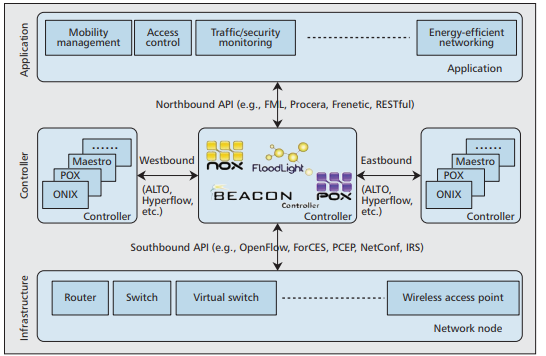
\includegraphics[scale=0.8]{Imagens/ArquiteturaSDN.png}
    \legend{Fonte: \citeonline{Sezer}}
    \label{ArquiteturaSDN.png}
\end{figure}
   
   \subsubsection{Camada de Infraestrutura}
   
   Também chamada de plano de dados ou de encaminhamento. Nesta camada concentram-se elementos de encaminhamento de pacotes, como switches(virtuais ou físicos) e roteadores, que devem ser programáveis e capazes de se comunicar com o controlador através das chamadas \emph{APIs SouthBound}. No paradigma SDN, apesar da existência de diversas \emph{APIs SouthBound}, o uso do Protocolo Openflow já é bastante difundido e tido como padrão para comunicação entre o plano de dados e de controle.\cite{kreutz} 

\subsubsection{Camada de Controle}

 Na camada de lógica e controle de dados, encontram-se os controladores, que são responsáveis por monitorar e modificar o comportamento dos dispositivos do plano de dados, tendo uma visão global da rede. Estes podem ser implementados em diversas linguagens e ainda serem conectados a outros controladores na mesma rede através das \emph{APIs Eastbound}, já as \emph{APIs Westbound} são responsáveis por prover comunicação entre dispositivos legados de rede. De modo a facilitar o gerenciamento e programação da rede, os controladores são vistos como sistemas operacionais de rede, pois utilizam uma interface de programação de alto nível para os operadores, abstraindo  a complexidade da camada de infraestrutura.\cite{McKeown:2008:OEI:1355734.1355746}
       
\subsubsection{Camada de Aplicação}

No nível mais alto da arquitetura temos a camada de aplicação ou gerenciamento, que se conecta com os controladores através das \emph{APIs Northbounds}. Essas interfaces são também importantes na arquitetura SDN, pois ao considerarmos os controladores como os sistemas operacionais da rede, podemos fazer uma analogia de que o mesmo necessita de outras aplicações que definam novas funcionalidades e serviços dentro do mesmo ambiente de acordo com a necessidade. Dessa forma, as aplicações de rede se tornam responsáveis de fato pelo controle lógico, cujos comandos serão traduzidos pelos controladores e enviados às entidades do plano de dados, ditando o comportamento dos mesmos.\cite{Nunes}
       
       Diferentemente da interface \emph{Southbound}, que utiliza de forma padrão o OpenFlow, essa interface ainda não possui uma proposta padronizada e comunicação entre os controladores e as aplicações que utilizarão seus serviços. De acordo com  \citeonline{kreutz}, ainda é cedo para essa padronização, pois os estudos de casos com as diferentes interfaces ainda estão ocorrendo. Contudo, é esperado que uma padronização venha a ocorrer com o desenvolvimento gradual do SDN. Além disso, as interfaces Northbound estão ligadas diretamente às implementações dos controladores, portanto, os diversos controladores existentes definem suas próprias interfaces para comunicação com a camada de aplicação. Mesmo que não seja o momento para definir uma interface \emph{Northbound} padronizada, existe o senso comum que para existir comunicação entre os diversos controladores é importante que essas interfaces sejam abertas e padronizadas, garantindo portabilidade e interoperabilidade. 
     

  
\par Diante da descrição das camadas e componentes de uma rede SDN, percebe-se que as vantagens desta quanto à separação do plano de dados e de controle se estende para diversos ambientes de rede, configurando soluções com aplicações para redes empresariais, \emph{data centers}, redes com infraestrutura \emph{wireless} e redes reais ou de pequeno porte.\cite{Nunes}


\subsection{O Protocolo OpenFlow}

%https://arxiv.org/pdf/1902.07913.pdf

%https://www.opennetworking.org/wp-content/uploads/2014/10/openflow-switch-v1.5.1.pdf

%https://books.google.com.br/books?id=ecM5CgAAQBAJ&pg=PT63&lpg=PT63&dq=role+controllers+sdn+master&source=bl&ots=mEkFEGV9AW&sig=ACfU3U3Hmiwz4MNiNYgl2HcoCGd_TA4J6Q&hl=pt-BR&sa=X&ved=2ahUKEwjowcH8n83nAhW0IbkGHX8cAm0Q6AEwEHoECAoQAQ#v=onepage&q&f=false



\subsection{Desafios em Redes SDN}

Os benefícios das redes SDN ainda contrastam com diversos desafios ocasionados pela própria arquitetura SDN. \citeonline{JAMMAL} em seu trabalho cita 8 desafios, ilustrados pela Figura \ref{Desafios.png}. 

\begin{figure}[!h]
    \caption{Desafios da arquitetura SDN.}
    \centering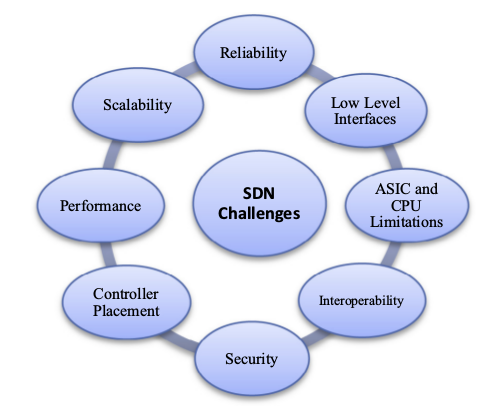
\includegraphics[scale=0.5]{Imagens/desafiosSDN.png}
    \label{Desafios.png}
    \legend{Fonte: \citeonline{JAMMAL}}
\end{figure}

\pagebreak

\begin{itemize}
    \item Confiabilidade: Em redes convencionais, quando há falha de algum dos dispositivos da rede o fluxo é desviado para outros dispositivos de forma a manter o fluxo. Entretanto, nas redes SDN a falha no controle lógico se torna um grande problema para o quesito confiabilidade, principalmente se esse controle está de fato centralizado em somente um controlador. 
    \item Escalabilidade: O desacoplamento dos planos de dados e de controle gera uma característica de interdependência na evolução das partes, contudo, também gera problemas na escalabilidade da rede. À medida que novos dispositivos físicos são inseridos e novos fluxos de rede são criados, o controlador pode passar a receber muito mais requisições do que pode processar, causando um "gargalo" na rede.
    \item Performance: A performance de uma rede SDN é medida por duas métricas: números de fluxos por segundo e tempo de configuração de fluxo. Para o caso do tempo de configuração de fluxo ainda existem os modos proativo e reativo, sendo que o último é normalmente utilizado pelo controlador SDN. Resumidamente, no modo reativo o tempo de configuração de fluxo é medido a partir do momento que o pacote chega no \emph{switch} e não há regras na tabela que especifiquem a ação sobre o mesmo. Dessa forma, o controlador toma alguma decisão sobre o pacote independente da tabela de fluxo. O tempo que o controlador leva para processar o pacote, tomar uma decisão e atualizar a tabela pode levar a problemas relacionados à latência e vazão.
    \item Posicionamento do controlador: A questão sobre a localização do controlador influencia em cada aspecto do plano de controle, seja nas latências dos fluxos até confiabilidade da rede e performance. O problema se resume em como posicionar um dado número de controladores numa certa rede física tal que suas funcionalidades sejam otimizadas para um objetivo específico.
    \item Limitações da CPU: As limitações da CPU no \emph{switch} afetam a banda entre este e o controlador. Esse quesito também afeta diretamente a questão da escalabilidade.
    \item Uso de interfaces de baixo nível entre controlador e dispositivos de rede: Apesar do SDN simplificar o gerenciamento de redes através das interfaces simplificadas para determinar políticas de rede de alto nível, o \emph{framework} das camadas inferiores precisam traduzir essas políticas para configurações de baixo nível no \emph{switch}.
    \item Segurança: A separação do plano de dados e controle tornou o gerenciamento de redes mais simplificado e dinâmico, contudo a segurança não é um quesito embutido nas características da arquitetura. Além disso, as tecnologias atuais de segurança foram pensadas especificamente para redes convencionais e justamente por ser um paradigma emergente, as redes SDN ainda não estão totalmente padronizadas, gerando ainda mais desafios para o quesito segurança.
    
\end{itemize}


\section{Conceitos de Segurança de Redes}

\par Gerenciar redes de computadores em um cenário com tantos usuários, grande volume de dados e diversidade tecnológica gerou novas vulnerabilidades nos sistemas, tornando-se um desafio para os pesquisadores da segurança de informação. Isso ocorre porque de acordo com \citeonline{kurose2010} uma comunicação para ser segura deve possuir as seguintes propriedades:

\begin{enumerate}
    \item \textbf{Confidencialidade}:  Indica que somente o remetente e o destinatário devem ter conhecimento do conteúdo da mensagem transmitida.
    
    \item \textbf{Autenticação de ponto final}: A comunicação deve ocorrer de forma que a identidade do remetente ou destinatário possa ser confirmada ou autenticada pela outra parte envolvida na comunicação.
    
    \item \textbf{Integridade de mensagem}: Deve-se garantir que a mensagem seja entregue sem alterações externas, mantendo a integridade da mesma até que o remetente possa ler a mensagem.
    
    \item \textbf{Segurança Operacional}: Redes com acesso à internet pública, principalmente redes corporativas, tornam-se vulneráveis para atacantes que a utilizam como forma de acesso à rede privada. Para este caso é importante que exista um sistema de detecção de atividade suspeita, sendo crucial para a segurança da informação.
    
\end{enumerate}

 Em um cenário onde exista troca de dados, as ameaças são inevitáveis. Uma ameaça é uma potencial violação da segurança, que ocorre quando existe uma circunstância, ação ou evento que possa gerar dano devido a uma vulnerabilidade, sendo intencional ou não.\cite{rfc2828}
 
 
 
\subsection{Segurança em Redes Definidas por Software}

\par Com o desenvolvimento das redes SDN e das tecnologias envolvidas, o estudo da segurança nessas redes tornou-se uma nova preocupação. Isso se deu porque o paradigma SDN se foca nas características operacionais da separação da camada de controle e de dados, deixando o quesito segurança como uma preocupação externa. Os desafios enfrentados quando se trata de SDN é que suas vulnerabilidades se encontram justamente nas suas principais características: programação de rede por software e centralização do controle lógico. \citeonline{kreutz} descreve em sua pesquisa sete ameaças potenciais nas redes SDN:

\begin{enumerate}
    \item Ataques por vulnerabilidades nos \emph{switches} OpenFlow: No nível do plano de dados, esse tipo de ataque a um \emph{switch} Openflow pode causar lentidão no fluxo, perda de pacotes, clonagem ou desvio de tráfego, além de ser possível injetar tráfego ou requisições falsas para sobrecarregar o controlador e \textit{switches} vizinhos.
    \item Fluxos de tráfego falsos: O atacante pode utilizar elementos físicos da rede para gerar ataques de DoS contra os \textit{switches} OpenFlow  e contra os controladores. 
    \item Ataques através do canal de comunicação do plano de controle e plano de dados: Esse ataque é feito direto no canal de comunicação entre o \textit{switches} e controladores para gerar ataques DoS ou para roubo de dados. A falha nesse caso se encontra no protocolo TLS/SSL, que por si só não garante confiabilidade no canal.
    \item Ataques por vulnerabilidades no controlador: Possíveis ataques por meio do controlador podem comprometer toda a rede justamente devido à centralização lógica do controle. Utilizar um mecanismo de detecção nesse caso pode não funcionar porque o próprio controlador pode mascarar seu comportamento por não existir um padrão fixo de eventos que o torne suspeito.
    \item Ausência de mecanismos de confiabilidade de comunicação entre controladores e aplicações: Análoga à ameaça 3, a preocupação se encontra na segurança do canal entre o controlador e as aplicações. 
    \item  Ataques por vulnerabilidades em estações administrativas: A falha em uma estação administrativa pode levar o atacante a acessar o controlador. Nas redes convencionais o princípio de tomar o controle é o mesmo, porém em uma rede a visão global da rede torna esse tipo de ataque ainda mais perigoso.
    \item Falta de recursos confiáveis para análise forense e remediação dos problemas: A detecção e remediação de uma ameaça não são garantidos se há falta de informações confiáveis dos elementos da rede.
\end{enumerate}

  Segundo \citeonline{rfc2828}, um serviço de segurança é um processo ou serviço de comunicação que fornece uma proteção específica para os recursos de uma rede. Entre esses serviços podemos citar serviços de autenticação, disponibilidade, auditoria, anonimização, entre outros. Para o cenário da arquitetura SDN, considerando as ameaças potenciais citadas e as comparando com as ameaças de redes convencionais, algumas soluções já foram propostas e desenvolvidas. Entre elas podemos citar o uso de módulos \emph{firewall}, serviços para controle de acesso, monitoramento e auditoria, proteção de privacidade, serviços para detecção de intrusos e melhoramento das políticas da rede SDN.\cite{ALSMADI}


\subsection{Anonimização de Redes}

Segundo \citeonline{rfc6235}, anonimização é a modificação dos dados em tráfego na rede de forma a proteger a identidade dos usuários finais. Para que isso ocorra é necessário que se remova a habilidade de identificar a conexão entre dois sistemas finais enquanto se protege a integridade dos dados. A anonimização é normalmente classificada de acordo com duas propriedades: recuperabilidade e contagem. Todas as técnicas de anonimização devem mapear identificadores ou valores em um espaço à parte, de acordo com alguma função específica. Caso essa função seja invertível, ou seja, caso seja possível recuperar o identificador ou valor real sem utilizar outra informações adicionais, então a técnica de anonimização utilizada é dita recuperável. Já a propriedade de contagem diz respeito à dimensão do espaço anonimizado e denota como a contagem de valores/identificadores únicos é preservado por uma função de anonimização.
\par O tráfego de dados, também conhecido como fluxo de rede, consiste em uma sequência de pacotes com origem e destino específicos. Esse fluxo é definido através de 5 campos: endereço IP de origem, endereço IP de destino, número da porta de origem, número da porta de destino e tipo de protocolo, sendo que ainda existem outros campos adicionais que identificam os pacotes e o fluxo a que pertencem. O processo de anonimização consiste justamente em proteger ou tornar anônimo dados que identifiquem unicamente os sistemas finais de origem ou destino \cite{farah}. A anonimização pode ser alcançada de forma geral por 4 modos: \cite{brekne}

  \begin{itemize}
      \item \textbf{Remoção de dados}: Implica na remoção de dados irreversível. Pode ser implementado substituindo os dados com uma constante;
      \item \textbf{Randomização}: Implica na substituição dos dados por uma informação aleatória.
      \item \textbf{Generalização}: Implica na substituição de dados por outros dados gerais. Caso esses outros dados identifiquem unicamente um usuário a anonimização pode falhar.
     \item \textbf{Truncamento}: Tipo de generalização em que um valor fixo de bits menos significativos  são deletados, enquanto o restante se mantém original.
  \end{itemize} 
  
  Atualmente já existem diversos algoritmos de anonimização que utilizam de forma geral um dos modos citados com algumas alterações. A Tabela \ref{tab1} ilustra alguns desses algoritmos.
  
 \begin{table}[h]
 \centering
 \caption{Algoritmos de anonimização}
\begin{tabular}{l | p{12cm}}

\hline 
\hline
\textbf{Campo} & \textbf{Algoritmos de anonimização} \\ \hline \hline
Endereço IP & Truncamento , Truncamento reverso, Permutação , Pseudoanonimização com preservação de prefixo, \emph{Black Marker} \\ \hline 
Endereço MAC &  Truncamento, Truncamento reverso, Permutação, Pseudoanonimização estruturada e \emph{Black Marker}\\ \hline
 Marcador Temporal & Degradação Precisa, Enumeração, \emph{Random-time shift}, \emph{Black Marker} \\ \hline
 Contador & Degradação Precisa, \emph{Random noise-addition}, \emph{Black Marker} \\ \hline
 Número da porta &  Permutação, \emph{Black Marker} \\ \hline

\end{tabular}
\label{tab1}
\legend{Fonte: Autoria própria}
\end{table}

A diferença desses algoritmos, além da implementação e sua eficiência, são os conjuntos de dados que são anonimizados.O algoritmo de \emph{Black Marker} é o método mais extremo, pois ele remove ou substitui todos os dados de um certo campo com valores fixados e pode servir para todos os campos. 
\par O algoritmo de enumeração se inicia após a ordenação dos dados. Ele seleciona o primeiro valor ordenado e escolhe um valor maior que este primeiro, de foma a adicioná-lo ao restante dos dados desse conjunto. 
\par O particionamento consiste em particionar um conjunto de possíveis valores em subconjuntos através de uma relação de equivalência de forma a selecionar um valor representativo dos conjuntos para substituir os dados.
\par A permutação é um algoritmo geralmente usado para os endereços IP e MAC. Ele aplica uma permutação aleatória ao conjunto de endereços a serem anonimizados com outro conjunto de endereços possíveis. Essa correspondência de endereços é feita através de uma tabela \emph{Hash}.

\par A pseudoanonimização com preservação de prefixo é similar à permutação e é utilizado para endereços IP. Neste caso o algoritmo procura preservar os n primeiros bits do endereço e utiliza criptografia para o restante dos bits.
\par O algoritmo \emph{Random-time shift} adiciona  um conjunto de valores aleatórios para todo valor em um campo.
\par O truncamento é utilizado também para endereços IP e MAC. Ele remove os \emph{n} bits menos significativos, os substituindo por 0. Já o truncamento reverso consiste na remoção dos \emph{n} bits mais significativos.
\par A técnica de degradação remove o conteúdo mais preciso de um marcador de tempo.

De acordo com \citeonline{Bomfim1} a maioria dos serviços de anonimização para redes SDN utiliza a técnica de deslocamento aleatório, contudo, a remoção ou substituição aleatória dos endereços IP inutiliza o pacote no sentido de não ser possível uma análise do fluxo. Também foi constatado em seu mapeamento que os endereços IP são os dados mais frequentemente anonimizados. Dessa forma, em seu mapeamento é proposto que se utilize a técnica de preservação de prefixo para endereços IP de forma a não inutilizar esses dados para análises de fluxo.

\subsection{Redes Autonômicas}

Lidar com a complexidade de sistemas e infraestruturas, bem como suas abstrações, sempre foi o maior desafio para a área da computação. De acordo com o artigo de \citeonline{horn}, pela IBM, o desenvolvimento de sistemas cada vez mais poderosos e complexos  tem o propósito de contribuir para a evolução humana em seus negócios e necessidades, portanto, a automação dos processos sempre fez parte do progresso. Entretanto, a crescente complexidade de Infraestrutura de TI, aliada à Internet como conhecemos, hoje chegou em um patamar de complexidade que ameaça estagnar os benefícios que a tecnologia pode oferecer. Essa complexidade também chegou aos administradores e usuários comuns gerando desafios também no quesito gerenciamento dessas tecnologias. Nesse contexto, \citeonline{horn} introduz a ideia de que a computação autonômica é último recurso possível para o progresso.
\par  A computação autonômica envolve o conceito de auto-gerenciamento do sistema a partir dos objetivos do administradores. O termo " autonômico" tem origem da biologia, através do conceito do sistema nervoso autonômico. Essa analogia se dá justamente porque o corpo humano possui um conjunto de sistemas altamente complexos que são interdependentes e se auto-gerenciam de acordo com fatores externos e internos.
\par As propriedades de um sistema autonômico são descritas na Tabela \ref{tab2}: \cite{RFC7575}:

\begin{table}[h]
 \centering
 \caption{Comparação entre conceitos da computação tradicional e autonômica.}
 \resizebox{\textwidth}{!}{%
\begin{tabular}{c | p{5cm} | p{5cm}}

\hline 
\hline
\textbf{Conceito} & \textbf{Computação Tradicional} & \textbf{Computação Autonômica} \\ \hline \hline
Auto-configuração & Os centros de dados corporativos possuem
vários fornecedores e plataformas. Instalar,
configurar e integrar sistemas é demorado e
propenso a erros. & A configuração automatizada de componentes e sistemas segue políticas de alto nível.
O resto do sistema se ajusta de forma automática e perfeita. \\ \hline 
Auto-otimização &  Os sistemas têm centenas de parâmetros
de ajuste não lineares configurados manualmente e seu número aumenta com cada versão. & Componentes e sistemas continuamente
buscam oportunidades para melhorar seu
próprio desempenho e eficiência. \\ \hline
 Auto-cura & A determinação de problemas em sistemas
grandes e complexos pode levar uma equipe
de semanas de programadores. & O sistema detecta, diagnostica e repara automaticamente problemas localizados de software e hardware. \\ \hline
 Auto-proteção &  A detecção e recuperação de ataques e falhas em cascata é manual.& O sistema defende automaticamente ataques mal-intencionados ou falhas em cascata. Ele usa aviso prévio para antecipar e
prevenir falhas no sistema. \\ \hline

\end{tabular} }
\label{tab2}
\legend{Fonte: Autoria própria}
\end{table}

Além das propriedades inerentes à arquitetura de um sistema autonômico, como descrito na Tabela \ref{tab2}, existem outras definições específicas para esse contexto de acordo com a RFC 7575 \cite{RFC7575}:

\begin{itemize}
    \item Intenção: Política abstrata de alto nível usada para operar a rede. É definida e fornecida por uma entidade centralizada.
    \item Domínio Autonômico: Um conjunto de nós autonômicos que instanciam a mesma intenção.
    \item Função Autonômica: Um funcionalidade ou função que não requere configuração e pode derivar todas as informações necessárias através do auto-conhecimento, descoberta ou intenção. 
    \item Agente de serviço autonômico: Agente implementado em um nó autonômico que também implementa uma função autonômica.
    \item Nó Autonômico: Um nó da rede que possui exclusivamente funções autonômicas e não requere nenhuma configuração. Pode ser exemplificado pelo roteador, \emph{switch}, PCs, entre outros.
    \item Rede Autonômica: Rede que contém exclusivamente nós autonômicos. Pode conter um ou vários domínios autonômicos.
\end{itemize}


